%
\hsection{\crowsFoot{I}{M1}{J}{M1}}%
\label{sec:rm:ij}%
%
\begin{figure}%
\centering%
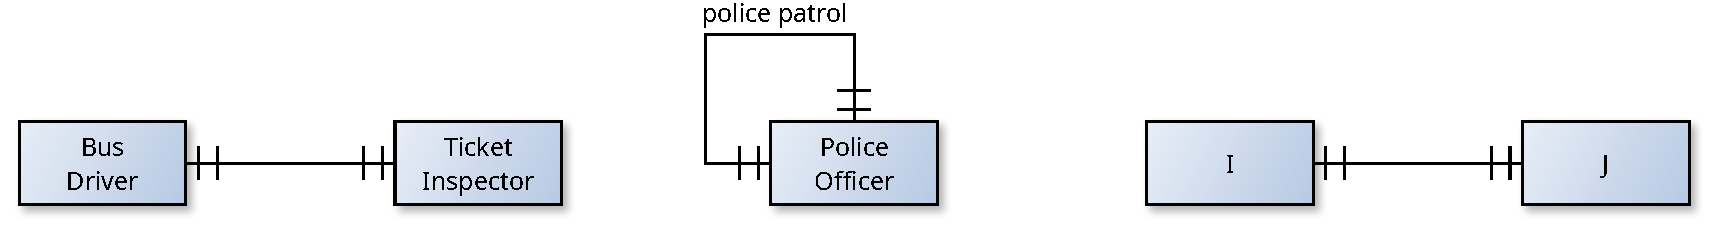
\includegraphics[width=0.97\linewidth]{\currentDir/IJ}%
\caption{Examples of the \crowsFoot{I}{M1}{J}{M1} relationship pattern from back in \cref{sec:conceptual:relationshipCardinalities}.}%
\label{fig:rm:ij}%
\end{figure}%
%
\gitSQL{\databasesCodeRepo}{conceptualToRelational/IJ_tables.sql}{IJ_tables}{%
The single-table realization of an \crowsFoot{I}{M1}{J}{M1} conceptual relationship.%
}%
%
We have the two entity types~I and~J.
Each entity of type~I must be linked to exactly one entity of type~J.
Each entity of type~J must be linked to exactly one entity of type~I.

We discussed a few examples of this relationship pattern from back in \cref{sec:conceptual:relationshipCardinalities}.
For example, in classical police movies or TV shows, there are always teams of two police(wo)men together performing a police patrol.
We can also imagine that there always is one bus driver working together with one ticket inspector together to service a bus route.
These examples are illustrated in \cref{fig:rm:ij}.

In this scenario, we only need a single table~\cite{S2024D:MEDTRDM}.
We just merge the attributes of the two entity types and put them all into one table.
If each pair of related entities of types~I and~J forms a single row in table~\sqlil{i_j}, then there can never be any issue with the referential integrity.
Neither can we have a row without the I~entity, nor can we have a row without entity of type~J.
This is illustrated in \cref{lst:IJ_tables}.
Since this is so very straightforward, we will not exercise inserting data into this table and selecting it back in another listing.%
%
\FloatBarrier%
\endhsection%
%
